\documentclass[titlepage]{jarticle}
\usepackage{h31ec-exp}
\usepackage[dvipdfmx]{graphicx}
\usepackage[yen]{okuverb}
\usepackage{here}

\title{LED点滅回路の製作}
\grade{3年40番}%
\author{鷲尾 優作}
\team{}
\date{令和3年5月17日}
\expdate{令和3年5月31日}
\coauthor{
  %26番 & 滝沢 倖大\\
  %31番 & 原山 蓮\\
  %34番 & 西脇 光
}

\begin{document}
\maketitle

%目次の出力
%\tableofcontents
%\newpage

\section{本実験の目的}
\begin{itemize}
    \item 電子部品に関する基礎知識や取り扱い方法を学ぶ.
    \item はんだごてやニッパなど工具の正しい使い方を再確認する.
    \item 簡単な電子回路の動作原理を理解する.
    \item 回路図を元に基板上での部品のレイアウトや実態配線を考える.
\end{itemize}

\section{理論}
図\ref{fig:回路構成図}に本実験で作成した回路の構成を示す.\\
回路はインバータ3素子,ICの入力に対する電流制限抵抗と発振周波数を制御するCR成分からなる発振部,
また発振回路によって生成された矩形波を用いて2つのLEDを交互に点滅させる点滅部,
平滑化コンデンサを含む電源部に大分される.

\begin{figure}[H]
    \begin{center}
        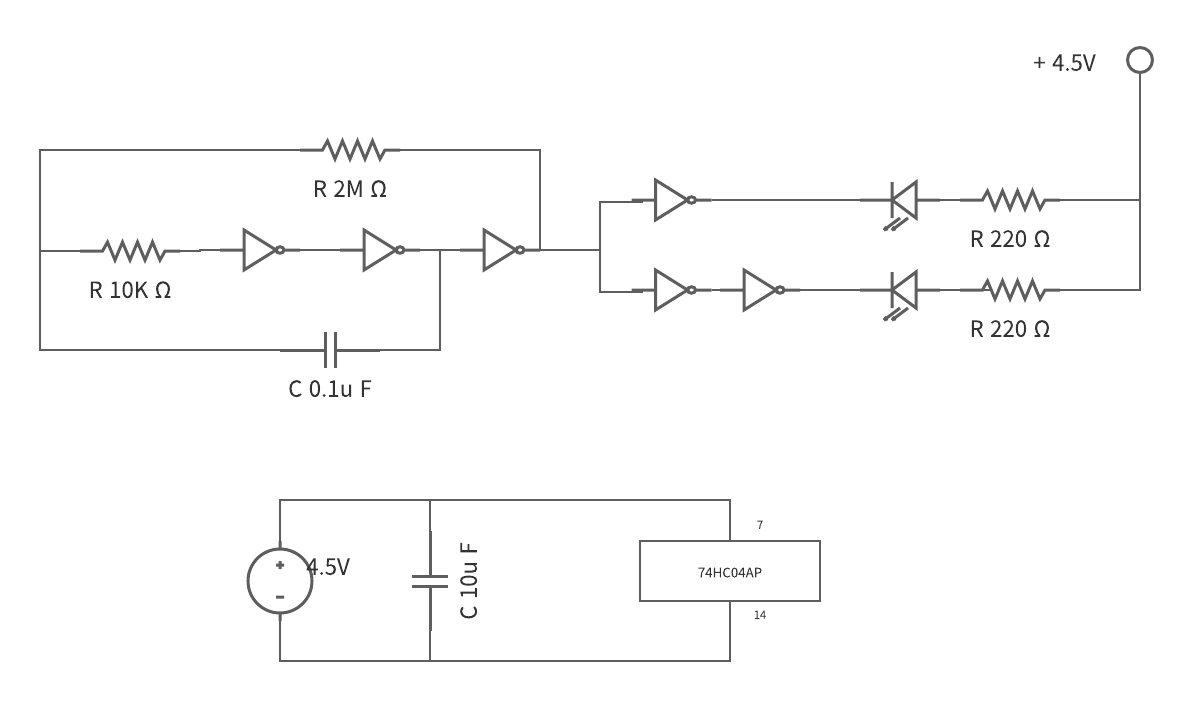
\includegraphics[width=10cm]{image/circuit.png}
        \caption{回路構成図}
        \label{fig:回路構成図}
    \end{center}
\end{figure}

各要素ごとに原理を示す.\\
\subsection{発振部}
ここではCの充放電により発生する波形を,インバータの入力端子の電位が変動することを利用し矩形波に変換している.\\
汎用インバータ74HC04APが出力する電流によりCが充電されるとC両端の電位差が上昇する.
これによりR10kΩを経由し最も源流に近いインバータが正負を反転し,続けて連続したインバータも反転する.
これによりCは周辺の電位が変動し,放電を開始する.放電によりC両端の電位差が下がれば,インバータの入力は再びLOWとなり回路の内部状態は
初期に復元する.

これにより,発振部はインバータの閾値Vthを境に逆転する矩形波を生成している.

また,点滅周期を高速にしたい場合\\
1. Cの静電容量を小さくする\\
2. R2MΩを小さくする\\
といった方法が考えられる.

この回路は日本庭園のししおどしとよく似た仕組みであるが,貯水する竹にあたる部分
すなわちC成分を小さくすれば発振速度は高速になる.2については竹に流入する水量,この場合は電流だがそれを増大させる
ため抵抗を小さくすることが有効である.

ただしICの出力電流には限界があるため特定の速度で頭打ちになるか,インバータの伝搬遅延時間の問題で高速化できなくなる点は
存在すると考える.

\subsection{点滅部}
この部分では片側のLEDを発生した矩形波の反転,もう片方のLEDを二重反転で制御することにより交互に点滅させている.\\
伝搬遅延時間は無視するものとして,入力された矩形波にしたがってLEDのカソードの電位をGNDにし点灯させている.同様にHIGHになっている
場合,ダイオードの両端に電位差は発生しないため消灯する.

課題に関連して,点灯時にLEDに流れる電流を求める.\\
キルヒホッフの電圧則より流れる電流を$I$とすると
\begin{eqnarray}
    4.5-220I-2.3 &=& 0 [\mathrm{V}]\\
    I &=& 2.2/220 = 0.010 [\mathrm{A}] = 10 [\mathrm{mA}]
\end{eqnarray}
となり,10mAであるとわかる.上記電圧方程式は,インバータICの寄生ダイオードや入出力インピーダンス等を完全に無視しており
インバータの出力が完全なGNDであるのが理想状態として計算したものであるので実装段階においての理想状態を意識したものではない.

\subsection{電源部}
電源はLEDのアノードと汎用インバータICに接続され,回路の動作を担っている.\\
動作の安定化のため平滑化コンデンサとしてアルミ電解コンデンサを挿入しており,電源ノイズの減少や瞬間的に電源不足に陥った場合のバックアップとして
機能する.

\section{実験内容}
同回路の実体配線図の作成を行った上でユニバーサル基板上に実装,動作確認を行う.

\section{計測器具}
\begin{enumerate}
    \item オシロスコープ\\用途 矩形波観測のため\\商品名GWINSTEK GDS-1022
\end{enumerate}

\section{成果物}
図\ref{fig:実体配線図}に作成した実体配線図を示す.
\begin{figure}[H]
    \begin{center}
        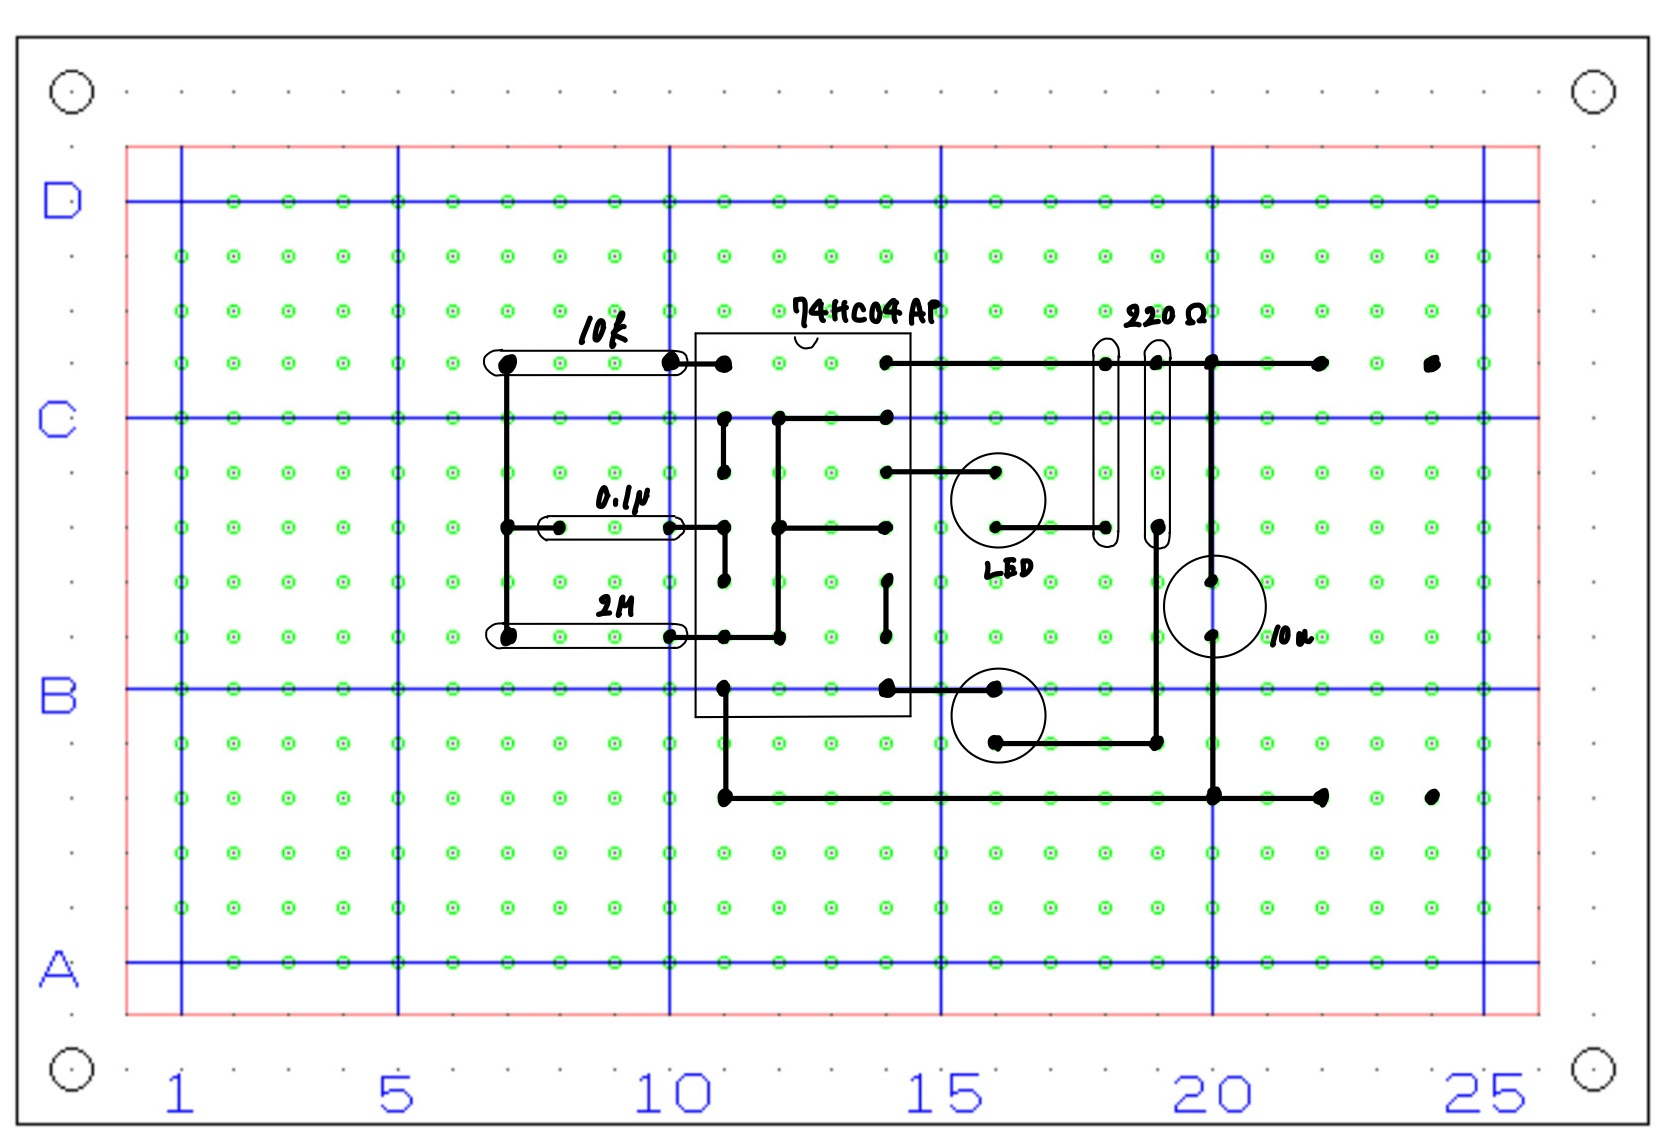
\includegraphics[width=10cm]{image/board.jpg}
        \caption{実体配線図}
        \label{fig:実体配線図}
    \end{center}
\end{figure}
今回の基板の配線設計では,各部品がどのような役割を持つか明確に分かるように位置を分け各部品が役割を果たせるよう配置した.
具体的にはLEDの電流制限抵抗を一か所に集め,発振周波数を決めるパラメータを回路左側に集中させ明確化したこと,
アルミ電解コンデンサを電圧源接続部と他部品との間に配置することで各部分に適切に平滑化後の電源がいきわたるよう設計したことがあげられる.

なお完全では無いが電源を横,信号を縦に配線するイメージを持ち作成することで初めて基板を見た人に親切になるよう意識した.

\section{動作確認}
初回動作確認時は汎用ICの型番が違っており予期せぬ動作があったが,はんだや配線に不良はなく無事に一度で完成することができた.
この時も予想外の動作があった時点で電源を遮断するなど適切な対応がとれた.ただしICの型番違いというミスに思い当たることができず
回路の配線ミスを疑ったことで時間的損失があった.

矩形波をオシロスコープで観測した際様子を図\ref{fig:確認風景}に示す.
\begin{figure}[H]
    \begin{center}
        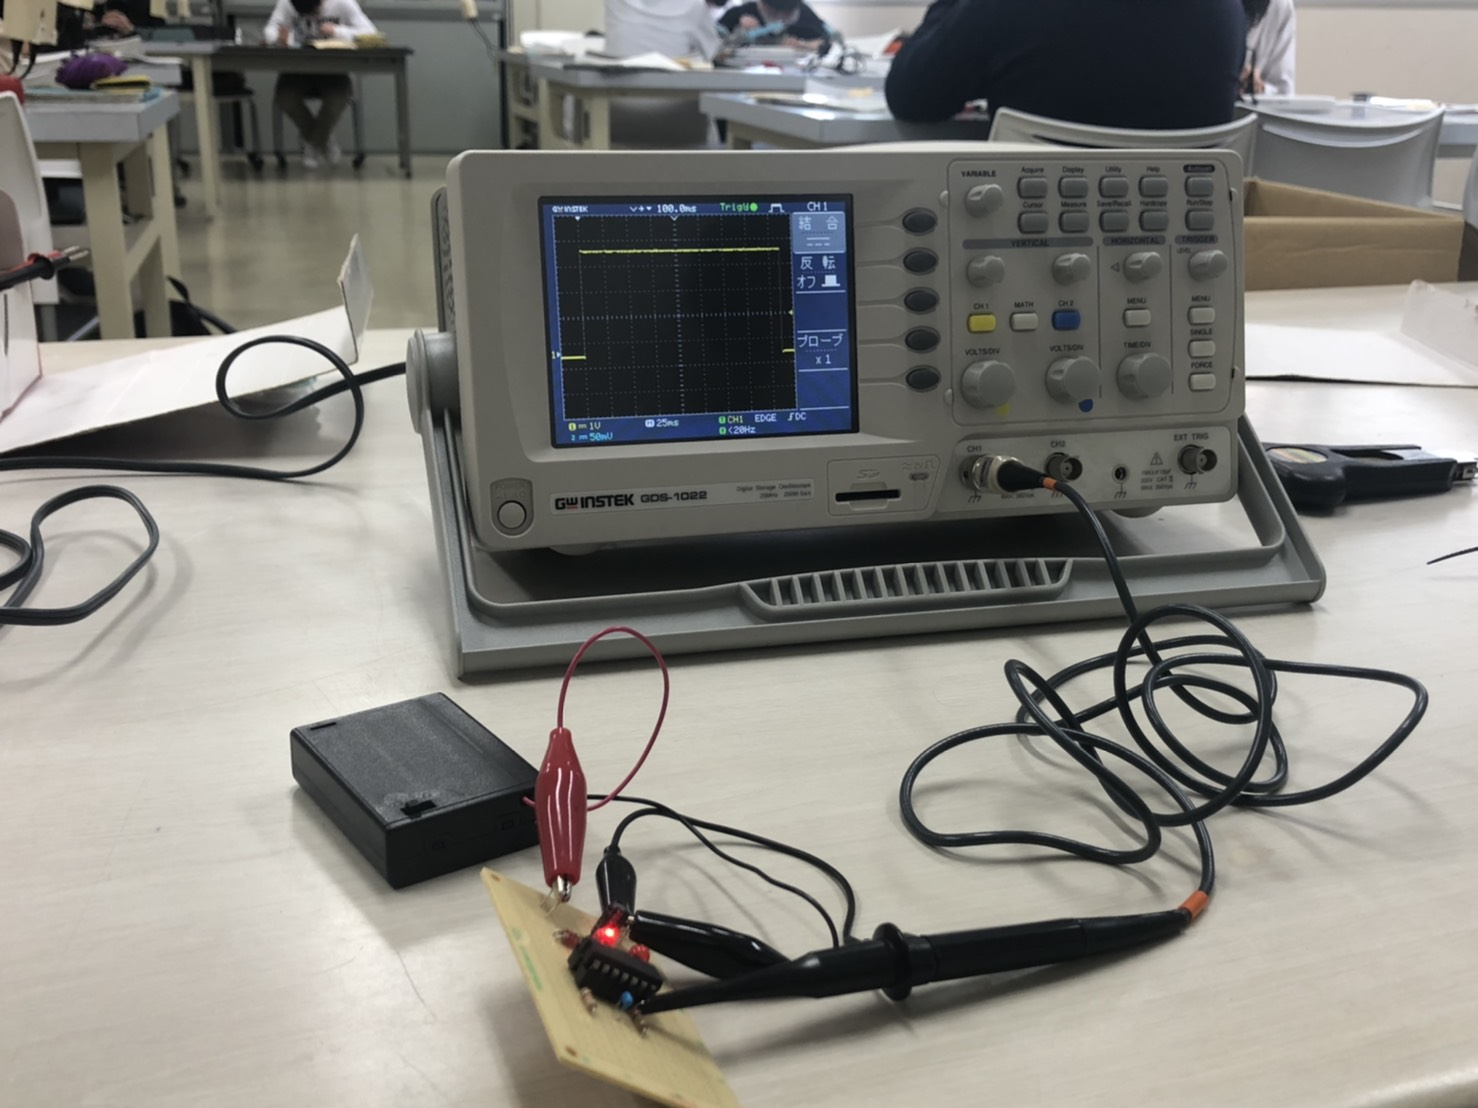
\includegraphics[width=10cm]{image/scope.jpg}
        \caption{確認風景}
        \label{fig:確認風景}
    \end{center}
\end{figure}
矩形波は1周期およそ425msであり,計算より発振周波数は
\begin{eqnarray}
    1/425 * 1000 \approx 2.35[\mathrm{Hz}]
\end{eqnarray}
であった.

\section{感想}
はんだずけを伴う実習も数回目となり,各所に配慮ができるようになってきた.今回の実験では汎用ICの型番違いによる基板検証が一番時間がかかりかつ
精神的にも良い結果にはならなかった部分だった.型番が違っていたので交換しにきたと伝えられるまでその可能性に気づけなかったこと,また自分以外にも同様の
異常がおきたとき与えられた回路自体を先に疑い型番なぞ気にも留めなかったことが今回の最大のミスだと考えている.
また,オシロスコープの測定があることが分かっていたにも関わらず測定点をICによって隠れやすい場所に配置してしまったのもマイナス要素であった.
同じ配置にしたとしてもテストピンを出すなど多少の配慮をするべきだったかもしれない.
結果的に決められた時間内に実験を終了させ次回から確認するべき点を得られたので総合して自己評価としては良い実習だったと考える.

\end{document}